\section{แนวคิดและวิธีการดำเนินงาน}
\label{sec:methodology}

งานวิจัยนี้นำเสนอวิธีการสร้างกรณีทดสอบและข้อมูลทดสอบสำหรับ{\TestPath}ที่ครอบคลุมความสัมพันธ์ระหว่าง{\softwareComponent}ในรูปขอบ{\scg} 
ซึ่งได้จากการวิเคราะห์{\StaticInformation}ของ{\sourcecode}ภาษาจาวา แล้วจึงนำมาสร้างกรณีทดสอบตลอดจนข้อมูลทดสอบซึ่งสอดคล้องกับเงื่อนไขที่พบ
ดัง\figref{fig:methodologyoverview} ซึ่งมีแนวทางการดำเนินงานดังนี้

\begin{sidewaysfigure}
    \centering
    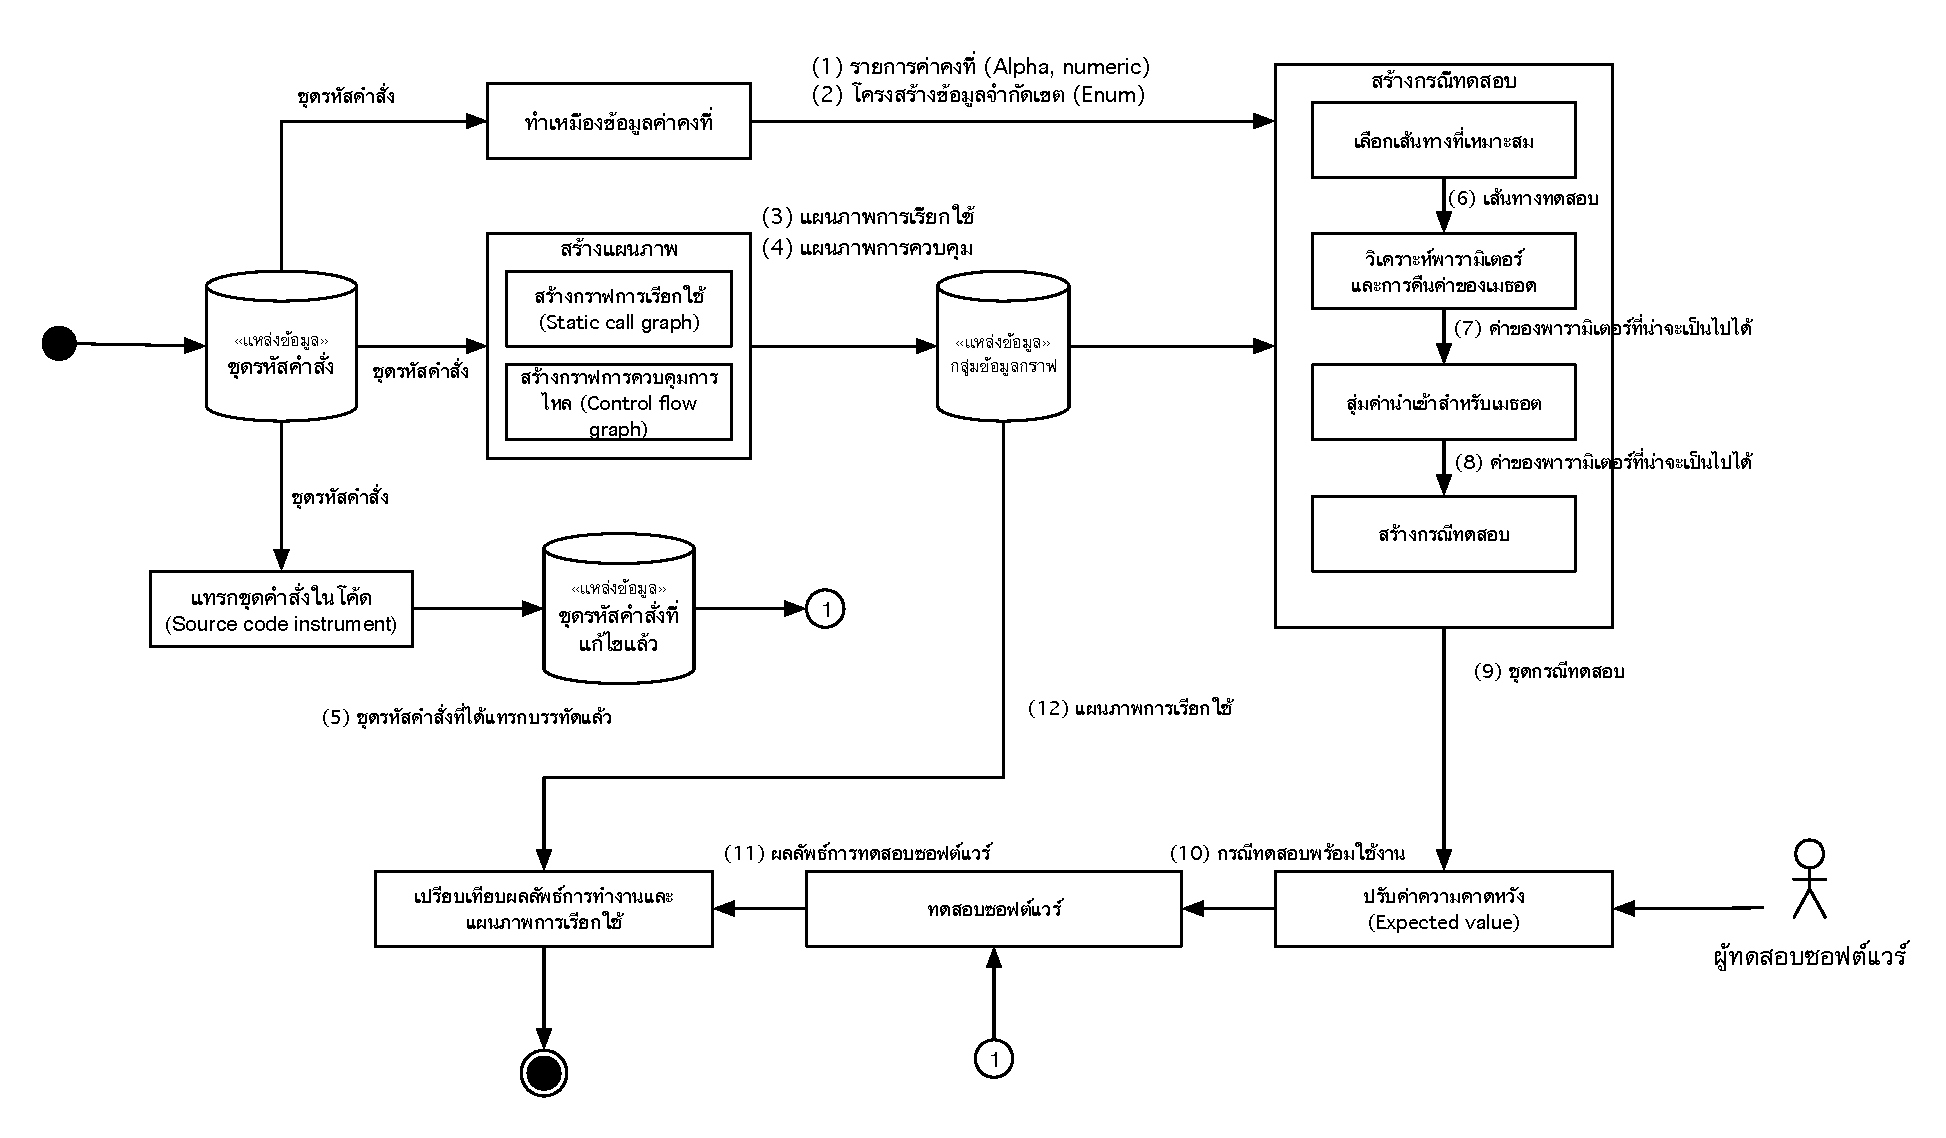
\includegraphics[width=0.9\textwidth]{methodology-overview}
    \caption{ภาพรวมการดำเนินงานวิจัย}
    \label{fig:methodologyoverview}
\end{sidewaysfigure}

% - - - - - - - - - - - - - - - - - - - -
\subsection{การวิเคราะห์ข้อมูลเบื้องต้น}
\label{subs:introsection}

ในขั้นตอนนี้เริ่มต้นด้วยการนำเข้าข้อมูล{\sourcecode}จาก{\Repository} เพื่อนำมารวบรวม{\StaticInformation} 
โดยสนใจเพียงเฉพาะ{\class}ซึ่งบรรจุอยู่ภายใน\FirstTimeDefine{\Package}{\PackageEN} ตามที่ผู้ใช้งานระบุ 
โดยกำหนดให้เป็น "\FirstTimeDefine{\CUT}{\CUTEN}" ทั้งนี้กระบวนการจะประกอบไปด้วย 3 ขั้นตอนด้วยกัน นั่นคือ
\FirstTimeDefine{\constantExtracting}, \FirstTimeDefine{\graphCreation}{\graphCreationEN} 
และ\FirstTimeDefine{\sourcecodeInstrumention}{\sourcecodeInstrumentionEN} 
โดยมีแนวทางการดำเนินงานของแต่ละขั้นตอน ดังนี้

% - - - - - - - - - - - - - - - - - - - -
% - - - - - - - - - - - - - - - - - - - -
\subsubsection{\constantExtracting}
\label{sec:sub:sub:sourceCodeExtract}

การทำเหมืองข้อมูลค่าคงที่นั้นเป็นกระบวนการเพื่อกำหนดแนวทางการในการสร้างข้อมูลทดสอบสำหรับ{\TestPath}ที่เลือก โดยมีแนวทางการจัดเก็บค่าคงที่ที่ประกาศไว้
ภายใน{\sourcecode} โดยสนใจกลุ่มข้อมูล 2 กลุ่ม ได้แก่

\begin{enumerate}
    \item {\it ข้อมูลพื้นฐาน (Primitive data)} ซึ่งเป็นข้อมูลพื้นฐานที่ใช้งานภายใน{\class} ซึ่งในที่นี้จะสนใจข้อมูลพื้นฐาน 2 ประเภทได้แก่
        \begin{enumerate}
            \item {\bf ตัวอักษร} ซึ่งมีประเภทข้อมูลเป็น \code{String} ในภาษาจาวา
            \item {\bf ตัวเลข} ซึ่งมีประเภทข้อมูล ได้แก่ \code{byte, short, int, long, float} และ\code{double} ในภาษาจาวา
        \end{enumerate}
    \item {\it โครงสร้างข้อมูลจำกัดเขต (Enumeration)} ซึ่งมีประเภทข้อมูลเป็น \code{enum} ในภาษาจาวา
\end{enumerate}

ทั้งนี้จะไม่สนใจข้อมูลเชิงตรรกะ (มีชนิดข้อมูลเป็น \code{bool} ในภาษาจาวา) เนื่องมาจากว่าตัวเลือกที่เป็นไปได้จำกัดอยู่แล้ว 
นอกจากนั้นจะยังไม่สนใจข้อมูลจำเพาะ ที่กำหนดขึ้นมาใช้งานเอง 
จาก{\sourcecode}ของ{\class} \code{SimpleBonusScore} และ\code{SimpleGrading} ดังที่แสดงใน 
\figref{fig:javaBonusScore} และ \ref{fig:javaGrading} ตามลำดับ ในการดำเนินการวิจัยครั้งนี้ 
จะจัดเก็บข้อมูลค่าคงที่ซึ่งอยู่ในบรรทัดที่ \code{6, 8, 9, 10, 11, 12, 15, 16, 17} และ \code{18} ของ{\class} \code{SimpleBonusScore}
ตลอดจนค่าคงที่ซึ่งอยู่ในบรรทัดที่ \code{4, 5, 6, 8, 9} และ \code{10} ของ{\class} \code{SimpleGrading} 
แล้วจึงนำมาจัดเก็บไว้ภายในฐานข้อมูลโดยแยกตาม{\class}ที่พบค่าคงที่เหล่านั้น เพื่อใช้ในขั้นตอน {\bf \testcaseGeneration} ต่อไป

หลังจากรวบรวม{\bf ค่าคงที่}จาก{\sourcecode}ได้เรียบร้อยแล้ว จะนำ{\bf ข้อมูลพื้นฐาน} และ{\bf โครงสร้างข้อมูลจำกัดเขต} ที่รวบรวมได้
จัดหมวดหมู่และบันทึกไว้ภายใน{\it ฐานข้อมูล}

% - - - - - - - - - - - - - - - - - - - -
% - - - - - - - - - - - - - - - - - - - -
\subsubsection{\graphCreation}
\label{sec:sub:sub:graphCreation}

กระบวนการสร้างกราฟนั้นจะรับข้อมูล{\sourcecode}จาก{\Repository}เพื่อนำข้อมูลมาใช้สร้างกราฟ โดยแบ่งออกเป็น 2 กระบวนการย่อยด้วยกัน 
นั้นคือ การสร้าง{\scg} และการสร้าง{\cfg} ดังนี้

\begin{enumerate}
    \item {\bf สร้าง{\scg}} อ่านข้อมูล{\CUT}ตามที่ผู้ใช้งานสนใจ แล้วนำมาสร้าง{\scg} โดยผลลัพธ์ที่ได้นั้นจะแบ่งเป็น 3 กลุ่ม ได้แก่
        \begin{enumerate}
            \item การเรียกใช้งานระหว่าง{\CUT}ด้วยกัน \label{ord:scgcut} 
            \item การเรียกใช้งานระหว่าง{\CUT}และ{\class}ภายในชุดพัฒนาของจาวา (Java SDK) \label{ord:scgjdk} 
            \item การเรียกใช้งานระหว่าง{\CUT}และชุดคำสั่งภายนอก (\code{3^{rd}} party library) \label{ord:scg3rd} 
        \end{enumerate}
        ซึ่งในแนวทางการดำเนินงานนี้จะสนใจเฉพาะ{\scg}ของ{\CUT}เท่านั้น ดังนั้นในขั้นตอนนี้ไม่สนใจกราฟที่เกิดจากการเรียกใช้ในข้อ 1.2
        และ 1.3 ตลอดจนกราฟที่เกิดจากการสร้างวัตถุใหม่ เพื่อให้ได้{\scg}เฉพาะ{\CUT} ดังเช่น{\scg}โปรแกรมคํานวณเกรดนิสิต ใน\figref{fig:scggrading}

    \item {\bf สร้าง{\cfg}} โดยจะอ่านข้อมูลของ{\CUT}นำมาสร้าง{\cfg}และจัดเก็บข้อมูลไว้ภายในฐานข้อมูล
\end{enumerate}

เมื่อสิ้นสุดกระบวนการจะนำข้อมูล{\bf {\scg}} และ{\bf {\cfg}} ที่ได้จัดเก็บลง {\it ฐานข้อมูล} เพื่อจัดเตรียมไว้สำหรับ 
{\bf ขั้นตอนการสร้างกรณีทดสอบ} และ{\bf เปรียบเทียบผลลัพธ์การดำเนินการ} ต่อไป

% - - - - - - - - - - - - - - - - - - - -
% - - - - - - - - - - - - - - - - - - - -
\subsubsection{\sourcecodeInstrumention}
\label{sec:sub:sub:srcInstrument}

เนื่องจากว่าการทดสอบนี้จำเป็นต้องครอบคลุม{\Path}ระหว่าง{\CUT} ดังนั้นจำเป็นจะต้องแทรกชุดคำสั่งใน{\sourcecode}ในแต่ละขั้นตอนการทำงาน 
จากนั้นจึงนำ{\sourcecode}ที่ผ่านการแทรกชุดคำสั่งเรียบร้อยแล้วไปใช้ในกระบวนการทดสอบ 
แล้วจึงจัดเก็บผลลัพธ์ที่ได้ระหว่างขั้นตอนการทดสอบ เพื่อนำมาเปรียบเทียบกับ{\TestPath}ที่เลือก

% \begin{figure}[ht!]
%     \lstset{style=thesiscodestyle}
%     \lstinputlisting[language=java]{methodology/SimpleBonusScoreInstrumented.java}
%     \caption{{\class} \code{SimpleBonusScoreInstrumented}}
%     \label{fig:javaBonusScoreInstrumented}
% \end{figure}
% 
% จากตัวอย่าง\figref{fig:javaBonusScoreInstrumented} เป็น{\sourcecode}ที่สืบเนื่องมาจาก\figref{fig:javaBonusScore}
% แต่ต่างกันโดยแทรกชุดคำสั่งเข้าไปภายใน{\sourcecode} ณ บรรทัดที่ \code{3, 6, 8, 11, 16, 19} และ \code{25} ซึ่งการแทรกชุดคำสั่งในกระบวนการนี้จะสนใจเพียงแค่{\CUT} เท่านั้น

เมื่อเสร็จสิ้นกระบวนการแทรกชุดคำสั่ง จะนำ{\sourcecode}ที่ได้จัดเก็บไว้ใน {\it ฐานข้อมูล} เพื่อจัดเตรียมไว้สำหรับนำไปทดสอบอีกครั้ง

% - - - - - - - - - - - - - - - - - - - -
\subsection{\testcaseGeneration}
\label{sec:sub:tcg}

การดำเนินงานวิจัยในครั้งนี้จะนำ {\bf ข้อมูลกราฟ} ซึ่งประกอบไปด้วย {\it {\scg}} ร่วมกับ{\it {\cfg}} ใช้เป็นข้อมูลเริ่มต้นเพื่อสร้าง{\TestPath}
ระหว่าง{\CUT} ให้ครอบคลุมความสัมพันธ์ระหว่าง{\class} ดังที่ปรากฎใน{\scg} โดยจะสร้างกรณีทดสอบโดยพิจารณาจาก{\PredicateNode}ที่ปรากฎบน{\TestPath}ที่เลือก 
สุดท้ายจึงนำข้อมูลทั้งหมดที่ได้สร้างเป็นชุดกรณีทดสอบ โดยมีภาพรวมการดำเนินงานดัง \figref{fig:testcaseGenerationActivity}

\begin{figure}[ht!]
    \centering
    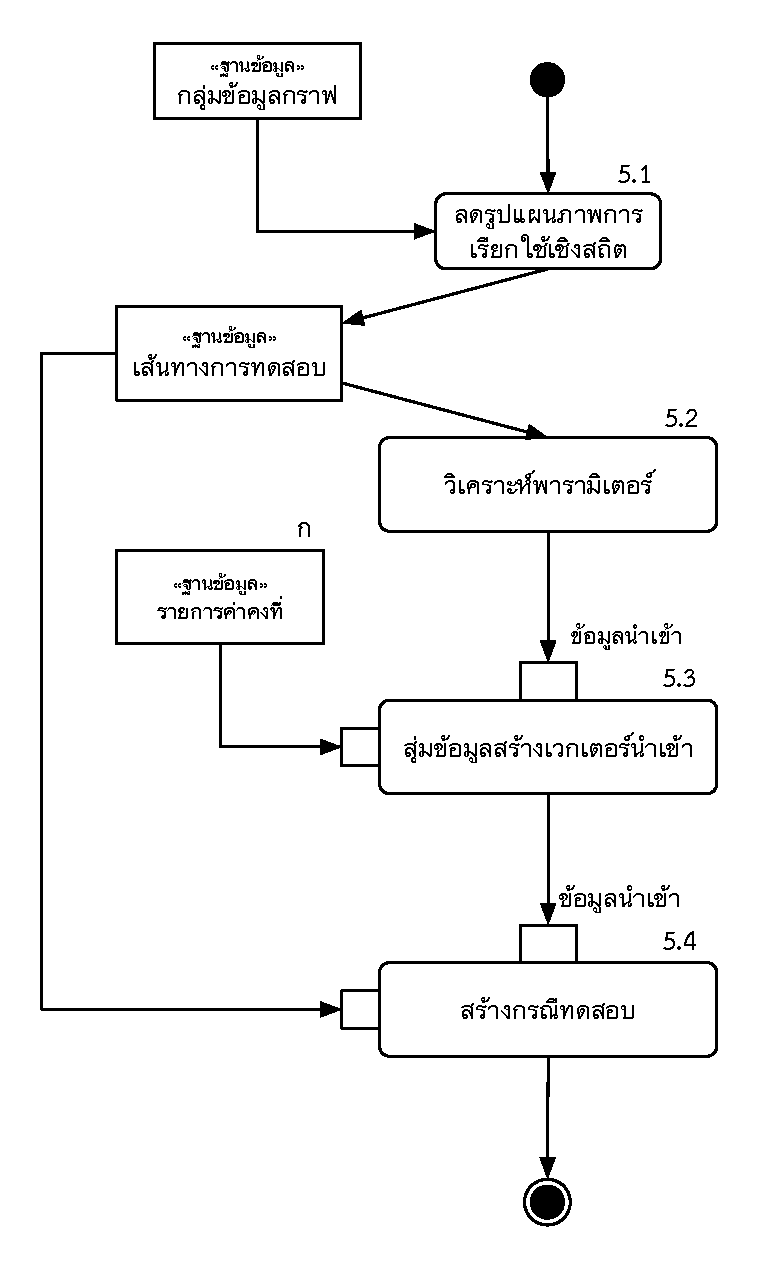
\includegraphics[width=0.5\textwidth]{methodology-activities-test-case-gen}
    \caption{ขั้นตอนการสร้างกรณีทดสอบ}
    \label{fig:testcaseGenerationActivity}
\end{figure}

% - - - - - - - - - - - - - - - - - - - -
% - - - - - - - - - - - - - - - - - - - -
\subsubsection{\testpathSelection}

ในขั้นตอนนี้จะพิจารณาจากข้อมูล{\it \scg} ร่วมกับ {\it \cfg} เพื่อเลือก{\TestPath}ที่ครอบคลุมความสัมพันธ์ระหว่าง{\class}ที่ปรากฎบน{\scg} 
เฉพาะระหว่าง{\CUT} ซึ่งจาก{\scg}ตัวอย่างใน\figref{fig:scggrading} จะได้{\TestPath} 2 {\Path} ด้วยกันคือ

\begin{enumerate}
    \item[\code{P_1:}] \code{G - [grading:score] - B - [score:getQuizScore] - Q}
    \item[\code{P_2:}] \code{G - [grading:score] - B - [score:getQuizSum] - Q}
\end{enumerate}

เพื่อให้ทราบถึงเงื่อนไขที่ทำให้กรณีทดสอบที่สร้างขึ้นสามารถทดสอบ{\TestPath}ข้างต้นได้ จึงใช้{\cfg}ของ{\method} \code{grading} จาก{\class} \code{SimpleGrading}, 
{\method} \code{score} จาก{\class} \code{SimpleBonusScore} รวมทั้ง{\method} \code{getQuizeScore} และ \code{getQuizSum} จาก{\class} \code{SimpleQuiz}
รวมพิจารณา ดัง\figref{fig:callreferences}

\begin{sidewaysfigure}[hbt!]
    \centering
    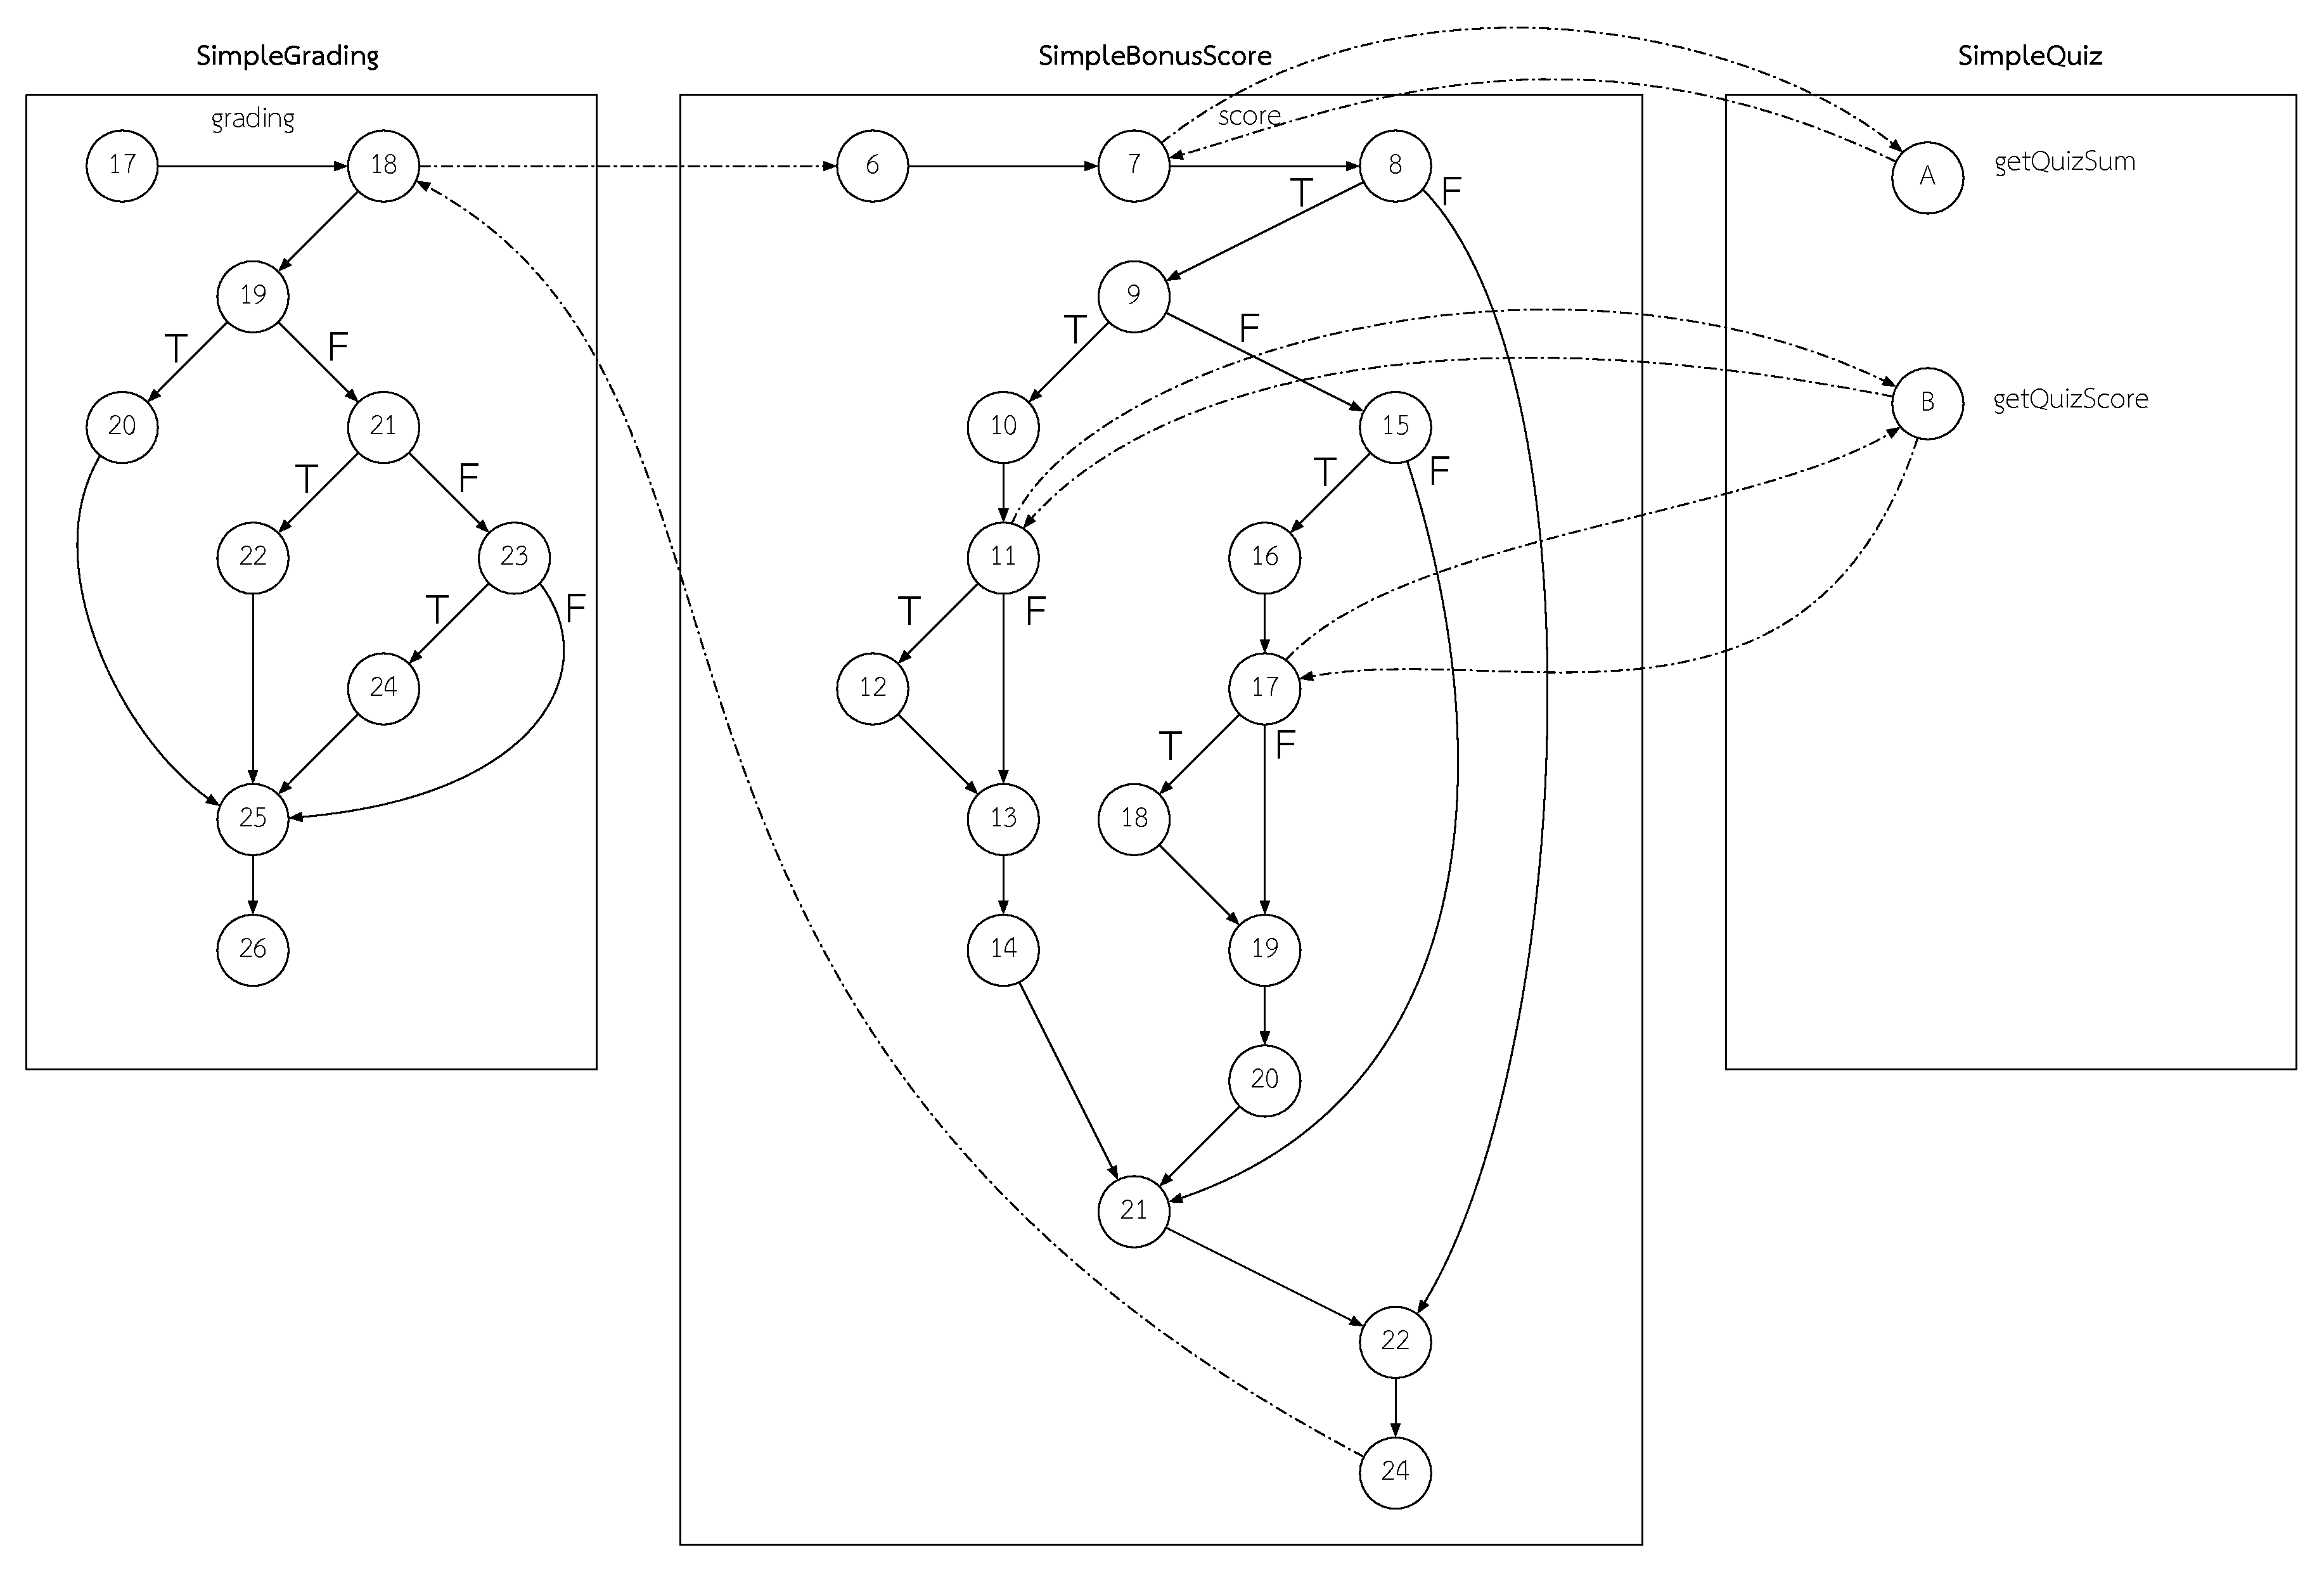
\includegraphics[width=0.9\textwidth]{test-path-selection-call-reference}
    \caption{โครงสร้างความสัมพันธ์ของ\class \code{SimpleGrading}, \code{SimpleBonusScore} และ\code{SimpleQuiz}}
    \label{fig:callreferences}
\end{sidewaysfigure}

ซึ่งมีแนวทางการเลือก{\TestPath} ดังนี้

\begin{enumerate}
    \item ให้น้ำหนักในทิศทางที่มุ่งไปยัง{\Node} ซึ่งพบการเรียกใช้งานระหว่าง{\class}ตามที่กำหนดไว้จาก{\scg}มากที่สุดเสมอ
    \item เลือก{\TestPath}ที่สั้นที่สุด (Shortest path) ก่อนเสมอ
    \item เลือก{\TestPath}ที่พบ{\PredicateNode}น้อยที่สุดก่อนเสมอ
    \item เลือก{\TestPath}ไปยังทิศที่ทำให้{\PredicateNode}มีค่าความจริงเป็นจริงก่อนเสมอ
\end{enumerate}

เมื่อพิจารณาข้อมูลกราฟดัง \figref{fig:callreferences} จะได้{\TestPath} \code{P_1} ดังนี้
\begin{equation*}
    \centering
    \code{P_1: \underbrace{17-18}_{G}-\overbrace{6-7}^{B}-\underbrace{A}_{Q}-\overbrace{7-\overline{8}-22-24}^{B}-\underbrace{18-19-20-25-26}_{G}} 
    \label{eq:exampleTestPathP1}
\end{equation*}
% \begin{equation*}
%     \centering
%     \code{P_2: \underbrace{17-18}_{G}-\overbrace{6-7-8-9-10-11}^{B}-\newline \underbrace{B}_{Q}-\overbrace{11-12-13-14-21-22-23-24}^{B}-\underbrace{18-19-20-25-26}_{G}}
% \end{equation*}

% - - - - - - - - - - - - - - - - - - - -
% - - - - - - - - - - - - - - - - - - - -
\subsubsection{การวิเคราะห์พารามิเตอร์และการคืนค่าของ{\method}}

แนวทางในขั้นตอนนี้จะนำ{\TestPath}ที่ได้คัดเลือกไว้ในขั้นตอนก่อนหน้านี้ (ซึ่งในที่นี้คือ \code{P_1} และ\code{P_2}) มาพิจารณาข้อมูลนำเข้า
และพารามิเตอร์ของแต่ละ{\method}ที่มีการเรียกผ่านกัน โดยจะเริ่มพิจารณาที่{\PredicateNode}ที่อยู่ในลำดับท้ายสุดของ{\TestPath}ก่อนเสมอ 
แล้วจึงนำเงื่อนไขการสร้างข้อมูลของทั้งเส้นทางมากำหนดกรอบสำหรับการสร้างข้อมูล 
ยกตัวอย่างเช่น \code{P_1} จะพบ{\PredicateNode}ทั้งสิ้น 2 {\Node} ด้วยกัน ได้แก่ {G: 19} และ \code{S: 8}
ซึ่งมีเงื่อนไขดังนี้

\begin{enumerate}
    \item[G:19] \code{student\_score < SCORE\_MINIMUM\_STATISFIED} \label{itm:studentscore}
    \item[S:8]  \code{bonus\_score > 0} \label{itm:studentid}
\end{enumerate}

โดยในขั้นตอนนี้จะนำค่าคงที่ที่เก็บไว้ในขั้นตอน {\bf \constantExtracting}} มาแทนในตัวแปร \code{SCORE\_MINIMUM\_STATISFIED} 
(\code{SCORE\_MINIMUM\_STATISFIED} มีค่าเท่ากับ \code{80}) แล้วจึงพิจารณาข้อมูลทดสอบจากเงื่อนไขข้างต้น
เพื่อสร้างกรณีทดสอบและข้อมูลทดสอบที่เข้าทดสอบ{\TestPath}ตามที่เลือกได้ โดยที่ข้อมูลที่สร้างขึ้นนั้นจะต้องทำให้เงื่อนไข 
\code{G:19} เป็นจริง (\code{True}) และเงื่อนไข \code{S:8} เป็นเท็จ (\code{False})

% - - - - - - - - - - - - - - - - - - - -
% - - - - - - - - - - - - - - - - - - - -
\subsubsection{\randomTestData}
\label{sec:sub:randomTestData}

สำหรับแนวทางการดำเนินงานในขั้นตอนนี้จะรับเงื่อนไขการสร้าง{\testData}จากกระบวนการก่อนหน้าเพื่อนำมาสร้างข้อมูลทดสอบ 
เพื่อให้กรณีทดสอบสามารถทดสอบ{\TestPath}ตามที่เลือกได้ ตามวิธีการที่กำหนด \cite{XING201491, Ma2016, Heaton2000} 
หากมีพารามิเตอร์ที่ไม่ปรากฎใน{\TestPath}เป็นข้อมูลนำเข้า ให้คำนวณหาค่าความน่าจะเป็นที่จะนำค่าคงที่มาใช้ TF-IDF 
(Term Frequency-Inverse Document Frequency: TF-IDF) \cite{Ma2016} 

เมื่อพิจารณาข้อมูล\FirstTimeDefine{\MethodSignature}{\MethodSignatureEN} ของ{\method} \code{score} ของ{\class} \code{SimpleGrading} 
พบว่า{\method}นี้ต้องการพารามิเตอร์ทั้งหมด 3 ค่า ด้วยกัน คือ \code{student\_id:String}, \code{student\_score:int} และ\code{bonus\_score:int} 
แต่จากตัวแปรที่พบใน{\PredicateNode}นั้นจะมีเพียง \code{student\_score} และ\code{bonus\_score} 
คงเหลือตัวแปร \code{student\_id} ที่จะใช้การคำนวณความคล้ายด้วยวิธี TF-IDF \cite{Ma2016}
กำหนดให้ค่าที่สุ่ม{\it \randomTestData } ได้ออกมาเป็นดัง \tabpageref{tab:GRTRandom}

\begin{table}[ht!]
    \centering
    \caption{ตัวอย่าง{\randomTestData}ที่ได้}
    \label{tab:GRTRandom}
    \begin{tabular}{|l|c|c|}
        \hline
        ตัวแปร                    & ประเภทข้อมูล   & ค่าที่สุ่มได้          \\ \hline
        \code{student\_score}    & {\it int}    & {\bf 75}         \\ \hline
        \code{bonus\_score}      & {\it int}    & {\bf 0}         \\ \hline
        \code{student\_id}       & {\it String} & {\bf "IUUUSISS"} \\ \hline
    \end{tabular}
\end{table}

% - - - - - - - - - - - - - - - - - - - -
% - - - - - - - - - - - - - - - - - - - -
\subsubsection{\testcaseGeneration}
\label{sec:sub:sub:tcGen}

ในขั้นตอนนี้จะนำข้อมูลนำเข้าที่สร้างจากกระบวนการก่อนหน้ามาสร้างกรณีทดสอบสำหรับภาษาจาวา โดยใส่{\expectedOutput} (บรรทัดที่ 7) 
จะเกิดจากการสุ่มโดยอิงตามประเภทข้อมูลที่{\method}นั้นคืนค่า ดังตัวอย่างของกรณีทดสอบภายใน {\it \testSuite} ดัง \figref{fig:junitGradingTest} ด้านล่าง

\begin{figure}[ht!]
    \lstset{basicstyle=\small,style=thesiscodestyle}
    \lstinputlisting[language=Java]{methodology/SimpleGradingTest.java}
    \caption{กรณีทดสอบที่สร้างขึ้นจากข้อมูลทดสอบ}
    \label{fig:junitGradingTest}
\end{figure}

% - - - - - - - - - - - - - - - - - - - -
\subsection{\expectedOutputAdjustment}
\label{sec:sub:expectedOutputAdj}

ในขั้นตอนนี้\tester จะทำหน้าที่ปรับค่า\FirstTimeDefine{\expectedOutput}{\expectedOutputEN}
แนวทางการดำเนินงานในขั้นตอนนี้จะเป็นการปรับค่าข้อมูลที่อยู่ภายในกรณีทดสอบที่ได้รับโดยนักทดสอบซอฟต์แวร์ เพื่อให้กรณีทดสอบนั้นสอดคล้องกับการทำงานที่ควรจะเป็นของโปรแกรม
มากที่สุด เนื่องจากการวิจัยครั้งนี้ยังไม่รองรับการวิเคราะห์ค่าผลลัพธ์ที่ได้จากการดำเนินงานของ{\method} ยกตัวอย่างเช่นกรณีทดสอบที่ได้จากขั้นตอนที่ 5.4 
ดัง \figref{fig:junitGradingTest} เมื่อได้ปรับการปรับค่าความคาดหวังจากนักทดสอบซอฟต์แวร์แล้วจะได้เป็นดัง{\figref{fig:junitGradingTestRefined}
ซึ่งในที่นี้นักทดสอบซอฟต์แวร์ได้ปรับค่าในบรรทัดที่ 5 โดยเปลี่ยนจาก \code{"IUUUSISS"} ให้เป็นค่า \code{"5873000021"} 
และบรรทัดที่ 7 คือค่า \code{"lorem"} เป็นค่า \code{"U"} จะได้ตัวอย่างของ {\it กรณีทดสอบพร้อมใช้งาน} ดังนี้

\begin{figure}[ht!]
    \lstset{style=thesiscodestyle}
    \lstinputlisting{methodology/SimpleGradingTest-Refined.java}
    \caption{กรณีทดสอบที่สร้างขึ้นจากข้อมูลทดสอบที่ปรับค่าจากนักทดสอบซอฟต์แวร์แล้ว}
    \label{fig:junitGradingTestRefined}
\end{figure}

\subsection{\executeSoftwareTesting}
\label{sec:sub:executeSoftwareTesting}

แนวทางการดำเนินงานในขั้นตอนนี้จะรับ {\it ชุดกรณีทดสอบ} เข้าทดสอบร่วมกับ{\sourcecode}ที่ผ่าน{\it \sourcecodeInstrumention} จาก{\it ฐานข้อมูล} 
และรวบรวมข้อมูลที่เกิดจากชุดคำสั่งที่แทรกไว้ ซึ่งปรากฎขึ้นระหว่างการทดสอบเข้าไว้ด้วยกันเป็น {\it ผลลัพธ์การทดสอบซอฟต์แวร์} 
เพื่อใช้ตรวจสอบให้แน่ใจว่ากรณีทดสอบนั้นสามารถทดสอบ{\TestPath}ที่เลือกได้ 

\subsection{\testResultCompare}

ในขั้นตอนนี้จะรับ {\it ผลลัพธ์การทดสอบซอฟต์แวร์} มาสร้างเส้นทางการทดสอบเทียบกับ{\TestPath}ที่ได้เลือกไว้ก่อนหน้านี้ 
เพื่อให้แน่ใจได้ว่าชุดทดสอบที่สร้างขึ้นนั้นครอบคลุม{\scg}ตาม{\TestPath}ที่กำหนดไว้
